\documentclass[10pt,a4paper,twocolumn]{article}

\usepackage[T1]{fontenc} % extended font encoding
\usepackage{enumerate} % lists
\renewcommand{\familydefault}{\sfdefault} % sans-serif
\usepackage{microtype} % better text justification
\usepackage{graphicx} % allow including pictures
\usepackage{color} % colors for pictures
\usepackage{fancyhdr} % headers and footers
\usepackage{titling} % picture in the title
\usepackage{hyperref} % clickable links
\usepackage{footnote} % footnotes in tables
\makesavenoteenv{tabular} % footnotes in tables
\usepackage[left=2cm,right=2cm,top=3cm,bottom=3cm]{geometry} % wider and taller page
\renewcommand*{\thefootnote}{\fnsymbol{footnote}} % use an asterisk for footnotes

\pagenumbering{gobble} % hide page numbers
\setlength{\columnsep}{1cm} % space between columns
\setlength{\parskip}{\baselineskip} % paragraphs divided by empty lines
\setlength{\parindent}{0pt}

\pdfinfo{
   /Author (Zlosynth Instruments)
   /Title  (Kaseta - Build Manual)
}

\pretitle{%
  \begin{center}
  \Huge
}
\posttitle{%
  \\
  \vspace{2cm}
  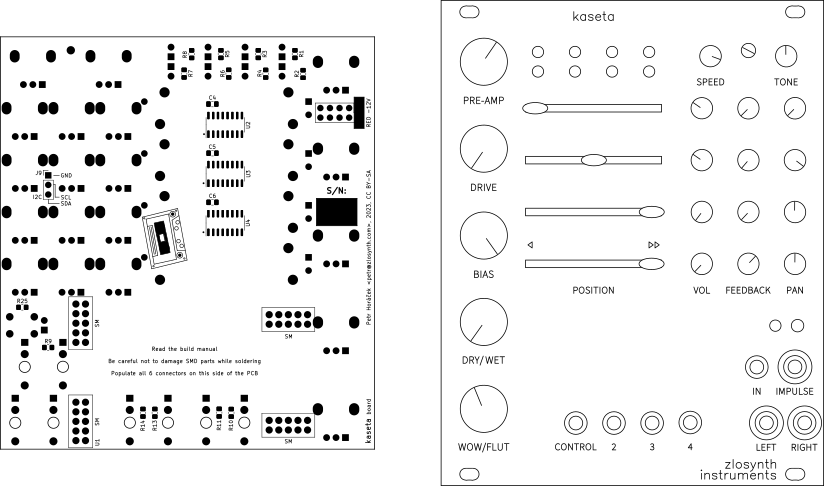
\includegraphics[width=16cm]{schema.pdf}
  \end{center}
}

\begin{document}

\title{Kaseta -- Build Manual}
\author{}
\date{}

\maketitle

\section{Overview}

You can always find the latest version of this build manual on
\url{https://zlosynth.com/kaseta-build-manual.pdf}.

This kit contains a printed circuit board (PCB) with all the surface mount
device (SMD) parts already pre-soldered. The through-hole components are left to
be assembled by you.

Pay attention to the orientation and position of all the parts. Desoldering them
would be difficult and may break the module. Also, use care not to touch the
pre-soldered SMD parts with the soldering iron. Read through the whole manual
first. Make sure you understand all the steps before you start soldering.

\newpage

\section{Tools required}

\begin{itemize}
  \item Soldering iron
  \item Masking tape
  \item Slotted head screwdriver
  \item Phillips head screwdriver
  \item Side-cutters
\end{itemize}

\newpage

\section{Bill of materials}

Start by unpacking all baggies into a bowl so you don't lose any components.

\begin{tabular}{@{}rl@{}}
  1 \texttimes & Front panel \\
  1 \texttimes & PCB (the black board) \\
  1 \texttimes & Daisy Patch Submodule (the yellow board) \\
  5 \texttimes & Blue trim potentiometer with center detent* \\
  9 \texttimes & Blue trim potentiometer without a detent \\
  1 \texttimes & Green D-shaped potentiometer with center detent* \\
  4 \texttimes & Green D-shaped potentiometer without a detent \\
  5 \texttimes & M7 nut and washer \\
  5 \texttimes & Knob \\
  4 \texttimes & Slider potentiometer and cap \\
  8 \texttimes & 3.5mm jack socket \\
  8 \texttimes & M6 nut and washer \\
  1 \texttimes & Tactile button \\
  9 \texttimes & Red LED \\
  1 \texttimes & Male connector 2\texttimes5 \\
  4 \texttimes & Female connector 2\texttimes5 \\
  1 \texttimes & Male connector 1\texttimes3 \\
  1 \texttimes & M2 slotted screw, M2 Phillips screw, standoff \\
\end{tabular}

* Potentiometers with a center detent snap when they are turned through their
center position.

\section{Power and I2C}

Start by soldering the power and I2C connectors.

\begin{enumerate}
  \item Take the male 2\texttimes5 connector and put the side with shorter legs
    through the footprint marked with a white stripe and a label ``RED~-12V''.
    Make sure to put it on the marked side of the PCB.
  \item Solder a single pin in and check that the connector is upright. If it
    is not, heat up the pin and align the connector by pushing it against the
    board.
  \item Solder all the pins in.
\end{enumerate}

Repeat the process for the male 1\texttimes3 connector, placed in the ``I2C''
footprint.

\section{Daisy Patch Submodule}

The Daisy Patch Submodule is connected to the main PCB through a set of
connectors.

\begin{enumerate}
  \item Mount the four female 2\texttimes5 connectors on the pins of the Daisy
    Patch Submodule. See Figure \ref{daisy}.
  \item Plug the mounted connectors into the black PCB through
    footprints marked as ``SM''. Make sure to put them on the correct side
    of the PCB, where all four connectors are marked.
  \item Solder all the pins in.
  \item Once done, carefully detach Daisy Patch Submodule to prevent it
    from getting damaged while progressing with the build. It may be a
    little difficult. Pull each connector by a millimeter at a time.
    The result is illustrated in Figure \ref{connectors}.
\end{enumerate}

\begin{figure}[h]
  \centering
  \includegraphics[width=\linewidth]{p01.jpg}
  \caption{All the components laid out}
\end{figure}

\begin{figure}[h]
  \centering
  \includegraphics[width=\linewidth]{p02.jpg}
  \caption{Connectors mounted on the submodule}
  \label{daisy}
\end{figure}

\begin{figure}[h]
  \centering
  \includegraphics[width=\linewidth]{p03.jpg}
  \caption{The power, I2C and submodule connectors}
  \label{connectors}
\end{figure}

\section{Front panel}

Now when all the internal parts are soldered, the next step is to assemble
parts sitting in the front panel.

\begin{enumerate}
  \item Put the hex standoff on top of the hole labeled ``Standoff'' and secure
    it there with the Phillips screw.
  \item Snap in the button.
  \item Place the 5 green D-shaped potentiometers in ``Green pot''
    footprints, do not solder them yet. The big legs on the sides are used to
    snap the pot in. Use the appropriate potentiometer for the bottom-most
    place marked as ``Green pot w/ center detent''.
  \item Similarly, place the 14 blue trimmer potentiometers in the ``Blue pot''
    footprints, some of which are marked for center detent.
  \item Place sliding potentiometers in their marked places. Do not put their
    caps on yet.
  \item Put all jack sockets into the PCB.
  \item Put LEDs in place. Pay attention to the markings on the PCB explaining
    their correct orientation.
  \item Now when all parts are in, carefully put the front panel on them.
    This is probably the most difficult part of this build. Be patient aligning
    all parts so they fit through holes. If you see that some are not getting
    through, use tweezers to align them. Leave the LEDs freely hanging in their
    holes for now.
  \item Put washers on the pots and jacks.
  \item Secure the front side of the standoff with the slotted screw. Tighten
    all the potentiometers and 3.5mm jack sockets in place with their nuts.
    Use care not to scratch the panel. Plastic tools are prefered,
    and steel drivers should also serve well. If you only have pliers, put them
    in a thick plastic bag. Protect the panel!
  \item Go over all the trimmer pots and check that they turn smoothly.
    Double-check that WOW/FLUT, TONE, and all four PAN potentiometers have a
    center detent.
\end{enumerate}

\begin{figure}[h]
  \centering
  \includegraphics[width=\linewidth]{p04.jpg}
  \caption{Backside before soldering}
  \label{Before soldering}
\end{figure}

\begin{figure}[h]
  \centering
  \includegraphics[width=\linewidth]{p05.jpg}
  \caption{Taped LED holes}
  \label{masking}
\end{figure}

\clearpage

Once all the components are placed correctly, move on to soldering.

\begin{enumerate}
  \item Solder in all the rotary potentiometers and jacks. Only solder the three
    smaller terminals of each potentiometer.
  \item For each sliding potentiometer, start by soldering one of its smaller
    terminals. After that, slide its shaft to the side of the just-soldered
    terminal. Then heat up the terminal while pressing on the shaft to make it
    sit flat on the PCB. Repeat the process on the other end of the
    potentiometer. Finally, solder the third small terminal.
  \item Use a masking tape on the portion of the panel with holes for LEDs, see
    Figure \ref{masking}. Push the LEDs against the tape, so they are even with
    the panel surface.
  \item Solder the LEDs. Then snap their legs off and remove the tape.
  \item Use tweezers to align the button. About 2 mm of it should be
    sticking out of the panel. Test that it can be easily clicked and
    returns to its resting position. If it does not, try to angle its body.
  \item Once the button is in a satisfying position, solder one of its legs,
    double-check it can be clicked and that it returns, and solder the remaining
    legs.
\end{enumerate}

\section{Knobs and caps}

You can now put knobs and caps on the potentiometers.

\begin{enumerate}
  \item Put black knobs on the five pots on the left. Align them with the
    D-shaped shaft and press them in. You may need to pull them a little bit if
    you see they are scratching the nut.
  \item Mount the black caps onto the shafts of slider potentiometers.
\end{enumerate}

\section{Final assembly}

Connect the Daisy Patch Submodule to the main black PCB to complete the build.

\section{Congratulations}

The module is now complete. Have fun!

You can find the user manual on \url{https://zlosynth.com/kaseta-user-manual.pdf}.

\vspace{2cm}

\begin{figure}[h]
  \centering
  \includegraphics[width=\linewidth]{p06.jpg}
  \caption{\centering Top, left, bottom and right side view of the assembled module}
\end{figure}

\begin{figure}[h]
  \centering
  \includegraphics[width=\linewidth]{p07.jpg}
  \caption{Front view of the assembled module}
\end{figure}

\end{document}
